\documentclass[sigconf,10pt,anonymous,review]{acmart}
\usepackage{booktabs}
\usepackage{tikz}

% HotStorage '26 submission template.
% Keep "anonymous,review" for submission. Remove them only for camera-ready.
% Official CFP: 5 pages for main text; references and appendix do not count.
% Titles must begin with either "Position:" or "Regular:".

\settopmatter{
  printacmref=false,
  printccs=false,
  printfolios=false
}
\renewcommand\footnotetextcopyrightpermission[1]{}
\pagestyle{plain}

\acmConference[HotStorage '26]{18th ACM Workshop on Hot Topics in Storage and File Systems}{September 28--29, 2026}{Prague, Czechia}
\acmYear{2026}
\copyrightyear{2026}
\acmDOI{}
\acmISBN{}

\begin{document}

% Replace Regular with Position if the paper is primarily a vision/argument paper.
\title{Regular: Cache Replacement for Realistic Multi-Tier Storage Workloads}

\author{Anonymous Author(s)}
\affiliation{
  \institution{Anonymous Institution}
  \country{}
}

\begin{abstract}
State the storage problem, the main empirical observation, the proposed idea,
and the strongest result in 120--150 words. For a HotStorage submission, the
abstract should make the ``hot topic'' angle obvious: what is changing in
storage systems, why existing approaches are now insufficient, and what your
paper contributes that the workshop audience can debate or build on.
\end{abstract}

\maketitle

\section{Introduction}
\label{sec:intro}
% Target length: 0.75--0.9 pages.
% Paragraph 1: concrete storage-system pain point.
% Paragraph 2: why prior cache replacement assumptions break.
% Paragraph 3: your key idea.
% Paragraph 4: contributions, preferably 3 bullets.

Modern storage stacks increasingly combine DRAM, flash, and remote or
disaggregated tiers, making cache replacement decisions more consequential than
they were in single-tier systems. This paper argues that replacement policy
should be evaluated under realistic object sizes, admission effects, write
amplification, and workload phase shifts rather than hit ratio alone.

This template is intentionally compact. Replace this text with your main
argument and keep the first page focused on motivation, novelty, and evidence.
Our contributions are:
\begin{itemize}
  \item We identify a workload property that makes conventional replacement
  policies fragile in modern storage caches.
  \item We propose a lightweight policy or measurement method that can be
  implemented in an existing cache simulator or prototype.
  \item We evaluate the method on trace-driven workloads and report both hit
  ratio and system-level costs.
\end{itemize}

\section{Motivation and Background}
\label{sec:motivation}
% Target length: 0.5--0.65 pages.
% Include one compact figure or table if it makes the problem vivid.

Use this section to establish the minimum context needed by a broad storage
audience. Define the cache hierarchy, the workload traces, and the evaluation
metric. Avoid re-teaching LRU; instead, explain the exact assumption your work
challenges.

\begin{figure}[t]
  \centering
  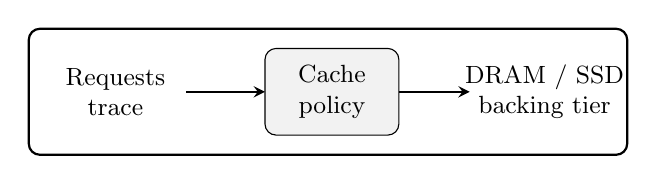
\begin{tikzpicture}[font=\small, >=stealth]
    \draw[rounded corners, thick] (0,0) rectangle (7.6,1.6);
    \node[align=center] at (1.1,0.8) {Requests\\trace};
    \draw[->, thick] (2.0,0.8) -- (3.0,0.8);
    \draw[rounded corners, fill=black!5] (3.0,0.25) rectangle (4.7,1.35);
    \node[align=center] at (3.85,0.8) {Cache\\policy};
    \draw[->, thick] (4.7,0.8) -- (5.6,0.8);
    \node[align=center] at (6.55,0.8) {DRAM / SSD\\backing tier};
  \end{tikzpicture}
  \caption{Use one simple figure to communicate the system model, not to
  decorate the page.}
  \label{fig:model}
\end{figure}

\section{Design}
\label{sec:design}
% Target length: 1.1--1.35 pages.
% Explain policy state, update path, eviction path, and overhead.

Describe the mechanism at the level where another systems researcher can
reimplement it. Keep pseudocode short and favor invariants over implementation
detail. If the paper is a position paper, rename this section to ``Argument''
or ``Research Agenda'' and use it to present the central thesis.

\subsection{Policy State}
State what metadata is stored per object, per queue, or per tier. Include the
byte overhead if the method will be compared to production policies.

\subsection{Replacement Decision}
Explain the admission and eviction decision path. Be explicit about what happens
on hits, misses, object resizing, and writeback.

\section{Evaluation}
\label{sec:evaluation}
% Target length: 1.1--1.3 pages.
% For HotStorage, preliminary but credible evidence is enough if the question is sharp.

Answer three questions:
\begin{enumerate}
  \item Does the idea improve the metric that matters for the target storage
  system?
  \item When does it fail or become equivalent to simpler policies?
  \item What is the overhead in metadata, CPU, or write amplification?
\end{enumerate}

\begin{table}[t]
  \centering
  \caption{Replace with your trace summary. Keep tables dense and factual.}
  \label{tab:traces}
  \begin{tabular}{lrrr}
    \toprule
    Trace & Requests & Objects & Read ratio \\
    \midrule
    A & 10M & 1.2M & 0.91 \\
    B & 25M & 3.7M & 0.76 \\
    C & 8M & 0.9M & 0.64 \\
    \bottomrule
  \end{tabular}
\end{table}

\section{Discussion and Limitations}
\label{sec:discussion}
% Target length: 0.45--0.6 pages.

Use this section to show judgment. Discuss deployment assumptions, interaction
with prefetching or admission control, sensitivity to trace bias, and why the
workshop should care even if the current prototype is incomplete.

\section{Related Work}
\label{sec:related}
% Target length: 0.3--0.45 pages in main text.
% Put citation-heavy detail in references, not prose.

Group prior work by idea, not by paper. For example: production cache
libraries, learned or adaptive replacement, flash-aware caching, and trace-driven
simulation. Cite representative papers such as CacheLib~\cite{berg2020cachelib}
and SIEVE~\cite{yang2024sieve}; add HotStorage papers that are closest to your
specific angle.

\section{Conclusion}
\label{sec:conclusion}
% Target length: 0.15--0.25 pages.

End with the storage-system implication, not a generic summary. A good
HotStorage conclusion makes the next experiment or debate obvious.

\clearpage
\bibliographystyle{ACM-Reference-Format}
\bibliography{references}

\appendix
\section{Appendix: Submission-Only Supporting Material}
Appendices are allowed by the 2026 CFP and do not count toward the 5-page main
text limit, but reviewers are not required to read them. Put only optional
details here: parameter sweeps, omitted proofs, or extra trace descriptions.

\end{document}
